\documentclass[11pt]{exam}
\usepackage[margin=1in]{geometry}
\pagestyle{plain}
\usepackage{amsmath,amsfonts,amssymb,amsthm,enumerate}
\usepackage{multicol}
\usepackage[]{graphicx}
\usepackage{hyperref}
\usepackage{tikz}
\usepackage{pgfplots}
\usepackage{subfigure}
\usepackage[final]{pdfpages}

\addtolength{\footskip}{2\baselineskip} % to lower the page numbers
\title{\vspace{-0.5in} Math 115 \\ Worksheet Section 5.1}
\date{}


% \theoremstyle{definition}
% \newtheorem{problem}{Problem}
\renewcommand{\questionlabel}{\textbf{Problem~\thequestion.}}
%\printanswers

\begin{document}
\maketitle
\vspace{-0.75in}
\begin{questions}
  \question The record time for the $100$ meter dash is $9.58$ seconds, set by Usain Bolt at a race in $2009$. Let $v(t)$ be Bolt's velocity, in meters per second, $t$ 
seconds after Bolt starts the race. Several values of $v(t)$ are shown below. 
\begin{center}
\begin{tabular}{|c|c|c|c|c|c|c|c|}
\hline
$t$ &0 & 0.5& 1& 1.5 & 2 & 2.5 & 3 \\
\hline
$v(t)$ & 0.6 & 3.5 & 5.8 &7.7  &9.1 &10.1 &10.6   \\
\hline
\end{tabular}
\end{center}
\begin{enumerate}[(a)]
\item Assume that Usain keeps his velocity constant in each of the
  intervals $[0,0.5)$, $[0.5,1)$, \([1,1.5)\), $[1.5, 2)$, $[2,2.5)$ and $[2.5,3)$. Compute the total distance Usain ran in the first $3$ seconds.

\item Now assume instead that Usain keeps his velocity constant in the
  intervals $(0,0.5]$, $(0.5,1]$, \((1,1.5]\) $(1.5, 2]$, $(2,2.5]$ and $(2.5,3]$ and compute the total distance he ran in this situation.

\item For each of the situations described in (a) and (b), make a sketch of the graph of the function $v(t)$. Can you represent each of the sums computed in (a) and (b) on the 
respective graph?
\end{enumerate}

Assume now that $v(t)$ is a continuous increasing function for the first three seconds of the race.

\begin{enumerate}[(a)]
\setcounter{enumi}{3}
	\item Based on the values provided on the table make a new sketch of $v(t)$.
	\item What information about the graph in (d) do the sums in (a) and (b) provide?
	\item Estimate the error when you compute the area below the graph of $v(t)$ using (a) and (b).
\end{enumerate}
\begin{solution}
  \begin{enumerate}[(a)]
  \item \(0.5(0.6+3.5+5.8+7.7+9.1+10.1) = 18.4\) meters
  \item \(0.5(3.5+5.8+7.7+9.1+10.1+10.6) = 23.4\) meters
  \item These are the piecewise functions whose area gives rectangles
    to estimate the area below the curve.
  \item 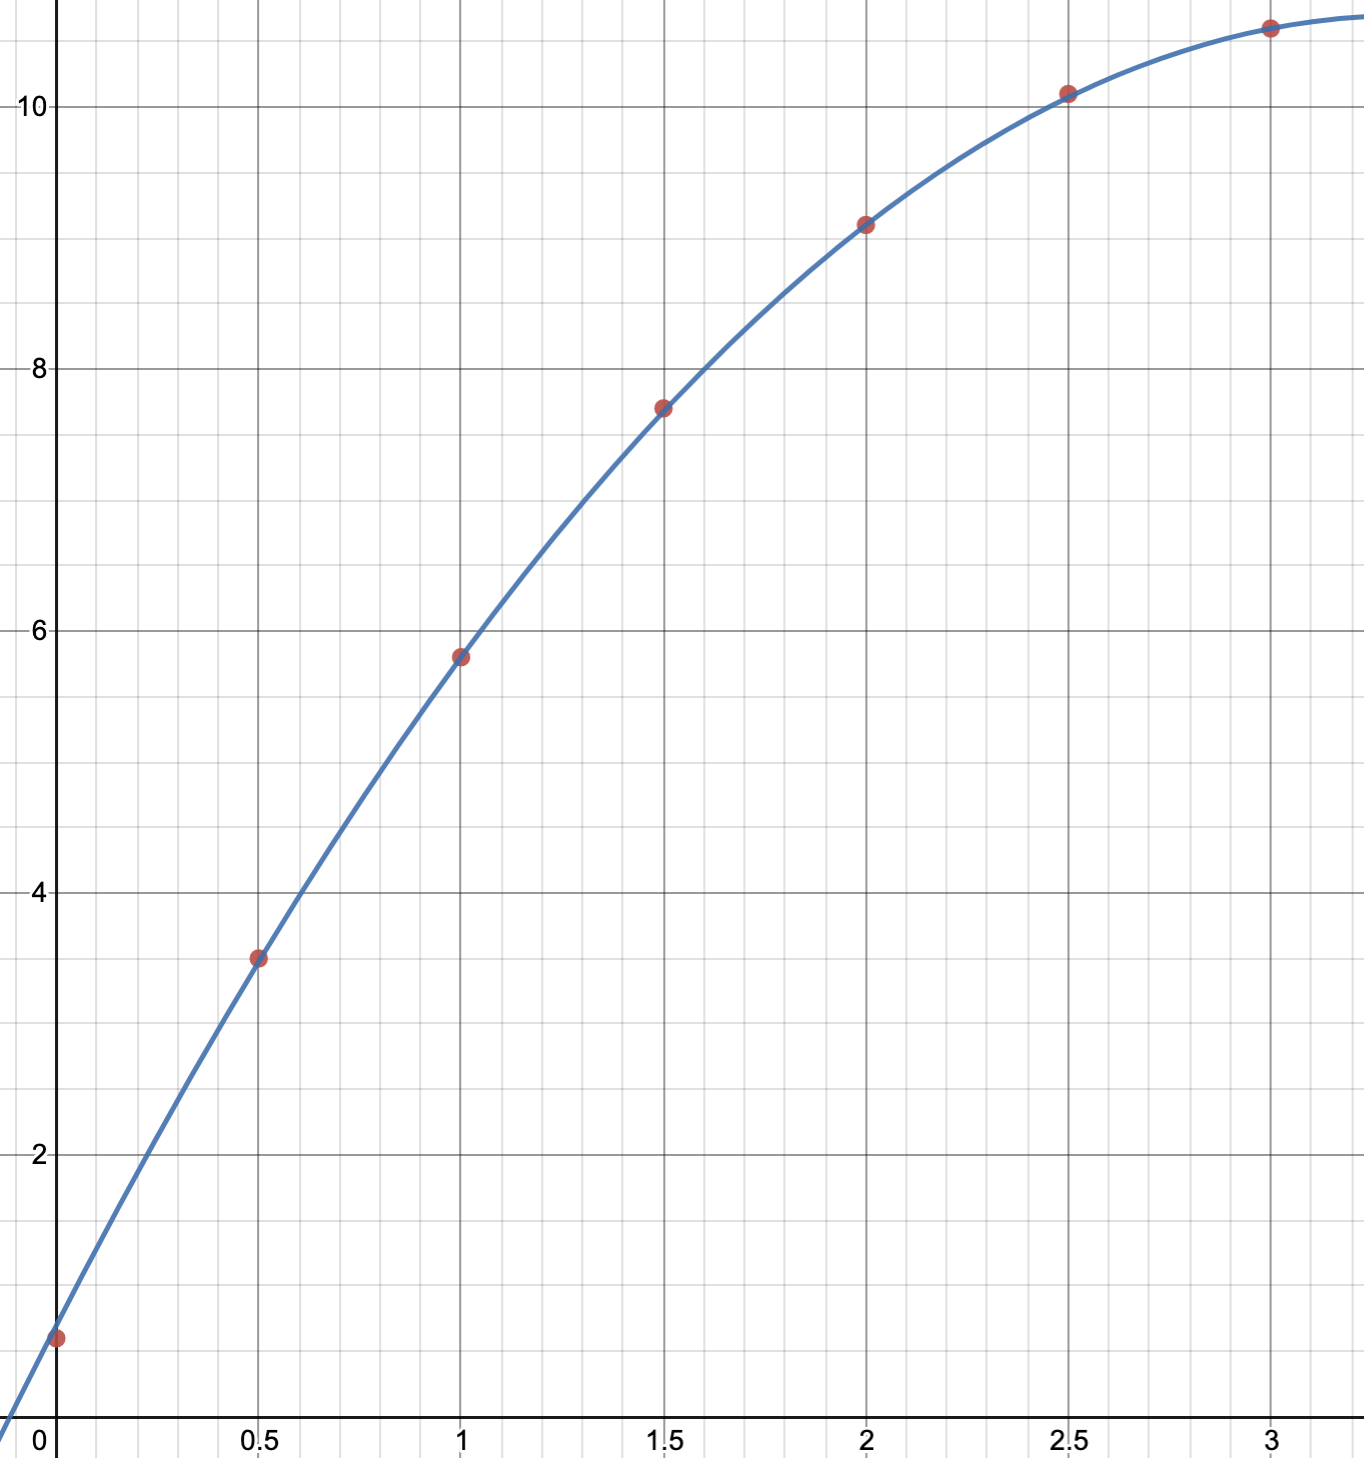
\includegraphics[scale=0.5]{Figures/1d}
  \item (a) represents the left-endpoint approximation of the area
    below the curve and (b)
    represents the right-endpoint approximation of the area below the curve.
  \item The error is probably about \(-2.5\) meters for (a) and \(2.5\)
    meters for (b). This is \(\frac{1}{2}\) the difference between the
    two estimates.
  \end{enumerate}
\end{solution}
\question The figure below shows the velocity of a car for $0 \leqslant t \leqslant 12$ and the rectangles used to estimate of the distance traveled.
  \begin{center}
 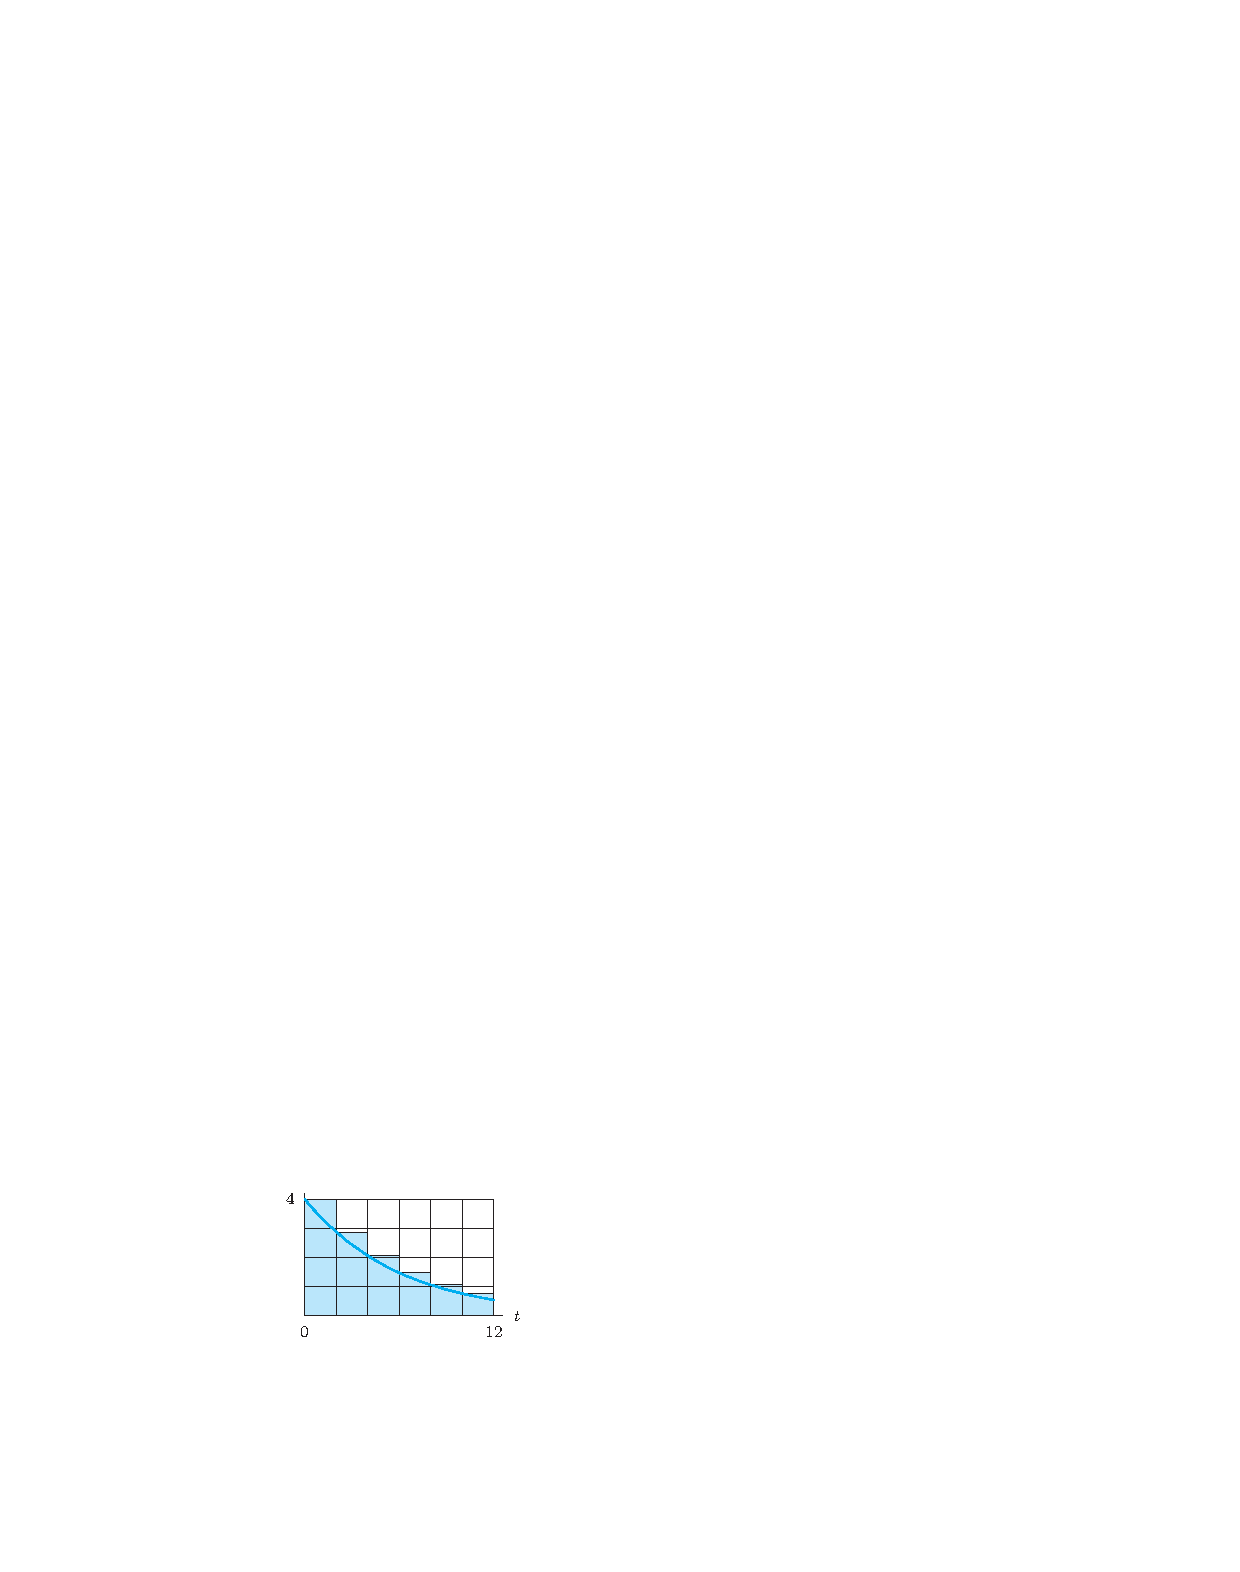
\includegraphics[scale=1.2]{Figures/fig2.pdf}
  \end{center}
\begin{enumerate}[(a)]
\item Do the rectangles represent a left or a right sum?
\item Do the rectangles lead to an upper or a lower estimate?
\item What is the value of $n$?
\item What is the value of $\Delta t$?
\item Give an approximate value for the estimate.
\end{enumerate}
\begin{solution}
  \begin{enumerate}[(a)]
  \item A left sum
  \item An overestimate
  \item \(n=6\)
  \item \(\Delta t = 2\) 
  \item \(2(4+2.9+2+1.5+1.1+0.8) = 24.6\)
  \end{enumerate}
\end{solution}
\question The velocity $v(t)$ in the table below is decreasing for $2 \leqslant t \leqslant 12$. 
\begin{center}
\begin{tabular}{|c|c|c|c|c|c|c|}
\hline
$t$ &2 & 4& 6& 8 & 10 & 12  \\
\hline
$v(t)$ &  44 & 42 & 41 & 40 & 37 & 35   \\
\hline
\end{tabular}
\end{center}

Using $n = 5$ subdivisions to approximate the total distance traveled, find

\begin{enumerate}[(a)]
\item An upper estimate.
\item A lower estimate.
\end{enumerate}
\begin{solution}
  \begin{enumerate}[(a)]
  \item 2(44+42+41+40+37) = 408
  \item 2(42+41+40+37+35) = 390
  \end{enumerate}
\end{solution}
\pagebreak
\question A particle's velocity is given by $v(t)$, where
\begin{equation*}
	\textnormal{(a)}\ \ v(t)=\begin{cases}
	2,&0\leqslant t\leqslant 3\\
	-8+2t,&3<t\leqslant 6
	\end{cases}\hspace{2cm}\textnormal{(b)}\ \ v(t)=3t^2,\ \ 0\leqslant t\leqslant 6.
\end{equation*}
\begin{enumerate}
	\item[(i)] For (a), compute the particle's displacement (signed area under the curve) between $t=0$ and $t=6$ using geometry.
	\item[(ii)]  For (b), estimate the displacement of the particle, using left and right sums with $n=6$.
\end{enumerate}
\begin{solution}
  \begin{enumerate}[(a)]
  \item We see that \(v(t)\) looks like the following graph with area
    shaded
    between the curve and the \(t\)-axis. \\

    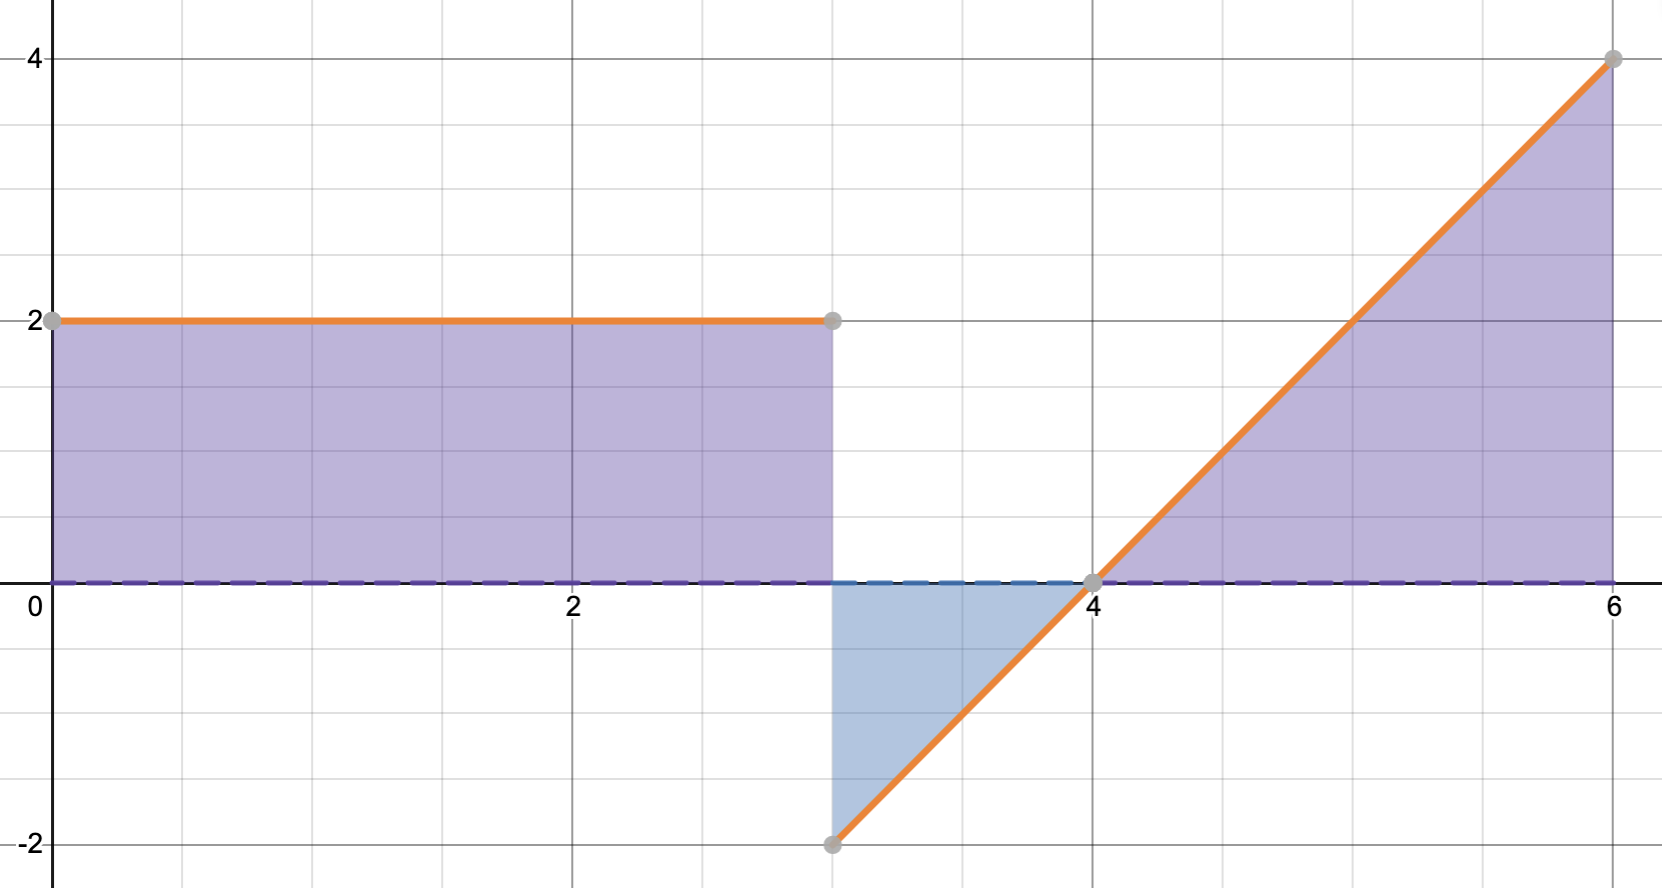
\includegraphics[scale=0.5]{Figures/prob4.png} To displacement, the purple
    portions contribute \(3(2)+0.5(2)(4) = 10\) and the blue portion
    contributes \(0.5(1)(-2) = -1\), so the displacement is
    \(10-1 = 9\).
  \item For (b), we create a table \\
    \begin{tabular}{|l|r|}
      \hline
      \(t\) & \(v(t)\)\\
      \hline
      0 & 0\\
      \hline
      1 & 3\\
      \hline
      2 & 12\\
      \hline
      3 & 27\\
      \hline
      4 & 48\\
      \hline
      5 & 75\\
      \hline
      6 & 108\\
      \hline
    \end{tabular}
    
    Then, a left sum gives us \(0+3+12+27+48+75 = 165\) and a right
    sum gives us \(3+12+27+48+75+108 = 273\).
  \end{enumerate}
\end{solution}
\question A bicyclist starts from home and rides back and forth along a straight east/west highway. Her velocity $y=v(t)$ at time $t$ (in minutes) 
measured  in feet per second is given below (positive velocities indicate travel toward the east, negative toward the west).
\begin{figure}[tbh]
\centering
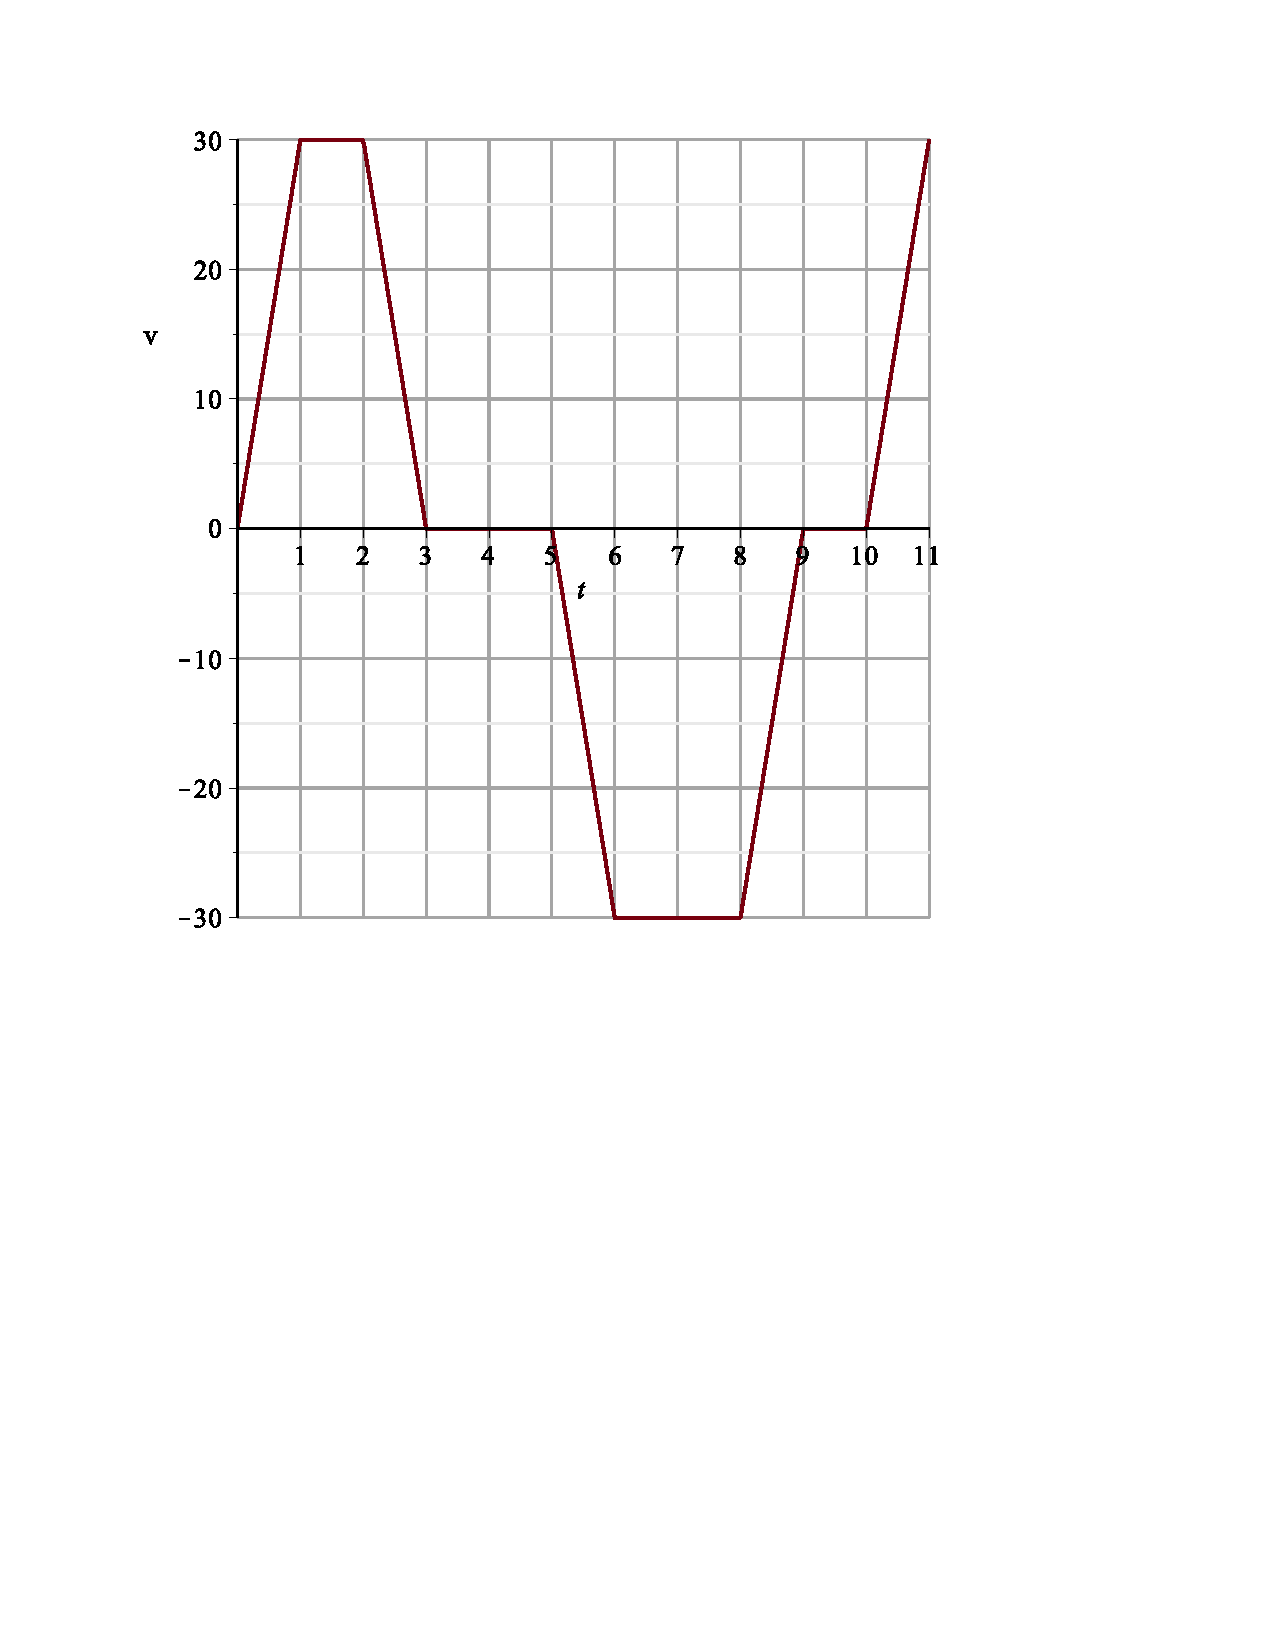
\includegraphics[scale=.5]{Figures/fig1.pdf}
\end{figure}
\begin{enumerate}[(a)]
	\item On what time intervals is she stopped?
	\item How far from home is she the first time she stops, and in what direction?
	\item At what time does she bike past her house?
	\item If she maintains her velocity at $t=11$, how long will it take her to get back home?
\end{enumerate}
\begin{solution}
  \begin{enumerate}[(a)]
  \item She is stopped on \((3,5)\) and \((9,10)\). 
  \item Notice that the time scale is in minutes but velocity is in
    feet per second. Also note that she first stops at \(t=3\). So, we
    must compute the area under the curve on \((0,3)\) and multiply by
    \(60\). This gives us \((15+30+15)\cdot 60 = 3600\) feet east.
  \item She bikes past her house at \(7.5\) minutes after she began
    since the signed area under the curve will be \(0\) at that point.
  \item At \(t=11\), the signed area is \(60-90+15 = -15\). So, it
    will take her another \(0.5\) minutes heading east at \(30\) feet
    per second to get home.
  \end{enumerate}
\end{solution}
\question The table below gives the expected growth rate, $g(t)$, in ounces per week, of the weight of a baby in its first $54$ weeks of life. Assume for this 
problem that $g(t)$ is a decreasing function. 
\begin{center}
\begin{tabular}{|c||c|c|c|c|c|c|c|}
\hline
week $t$ &0 & 9& 18& 27 &36&45 & 54 \\
\hline
growth rate $g(t)$ & 6 & 6 & 4.5 &3  &3 &3 &2   \\
\hline
\end{tabular}
\end{center}
\begin{enumerate}[(a)]
	\item Using six subdivisions, find an overestimate and an underestimate for the total weight gained by a baby over its first $54$ weeks of life.
	\item How frequently over the $54$ week period would you need the data for $g(t)$ to be measured to find overestimates and underestimates for the total weight gain 
over this time period that differ by $8$ oz?
\end{enumerate}
\begin{solution}
  \begin{enumerate}[(a)]
  \item Overestimate: \(9 (6+6+4.5+3+3+3) = 229.5\) ounces. Underestimate:
    \(9(6+4.5+3+3+3+2) = 193.5\).
  \item The difference between our estimates is \(9(6-2) = 36\). To
    get a estimates that differ by only \(8\) ounces, we would need
    \(\Delta t=2\) instead of \(\Delta t =9\). Since \(\Delta t =
    \frac{b-a}{n} = \frac{54}{n}\), the result is \(n = \frac{54}{2} =
    28\) measurements, one every 2 weeks.
  \end{enumerate}
\end{solution}
\question The following graphs show the velocity, in cm/sec, of a
  particle moving along a number line. Find the change in position and
  total distance traveled between times \(t=0\) and \(t=5\) seconds.
  \begin{center}
    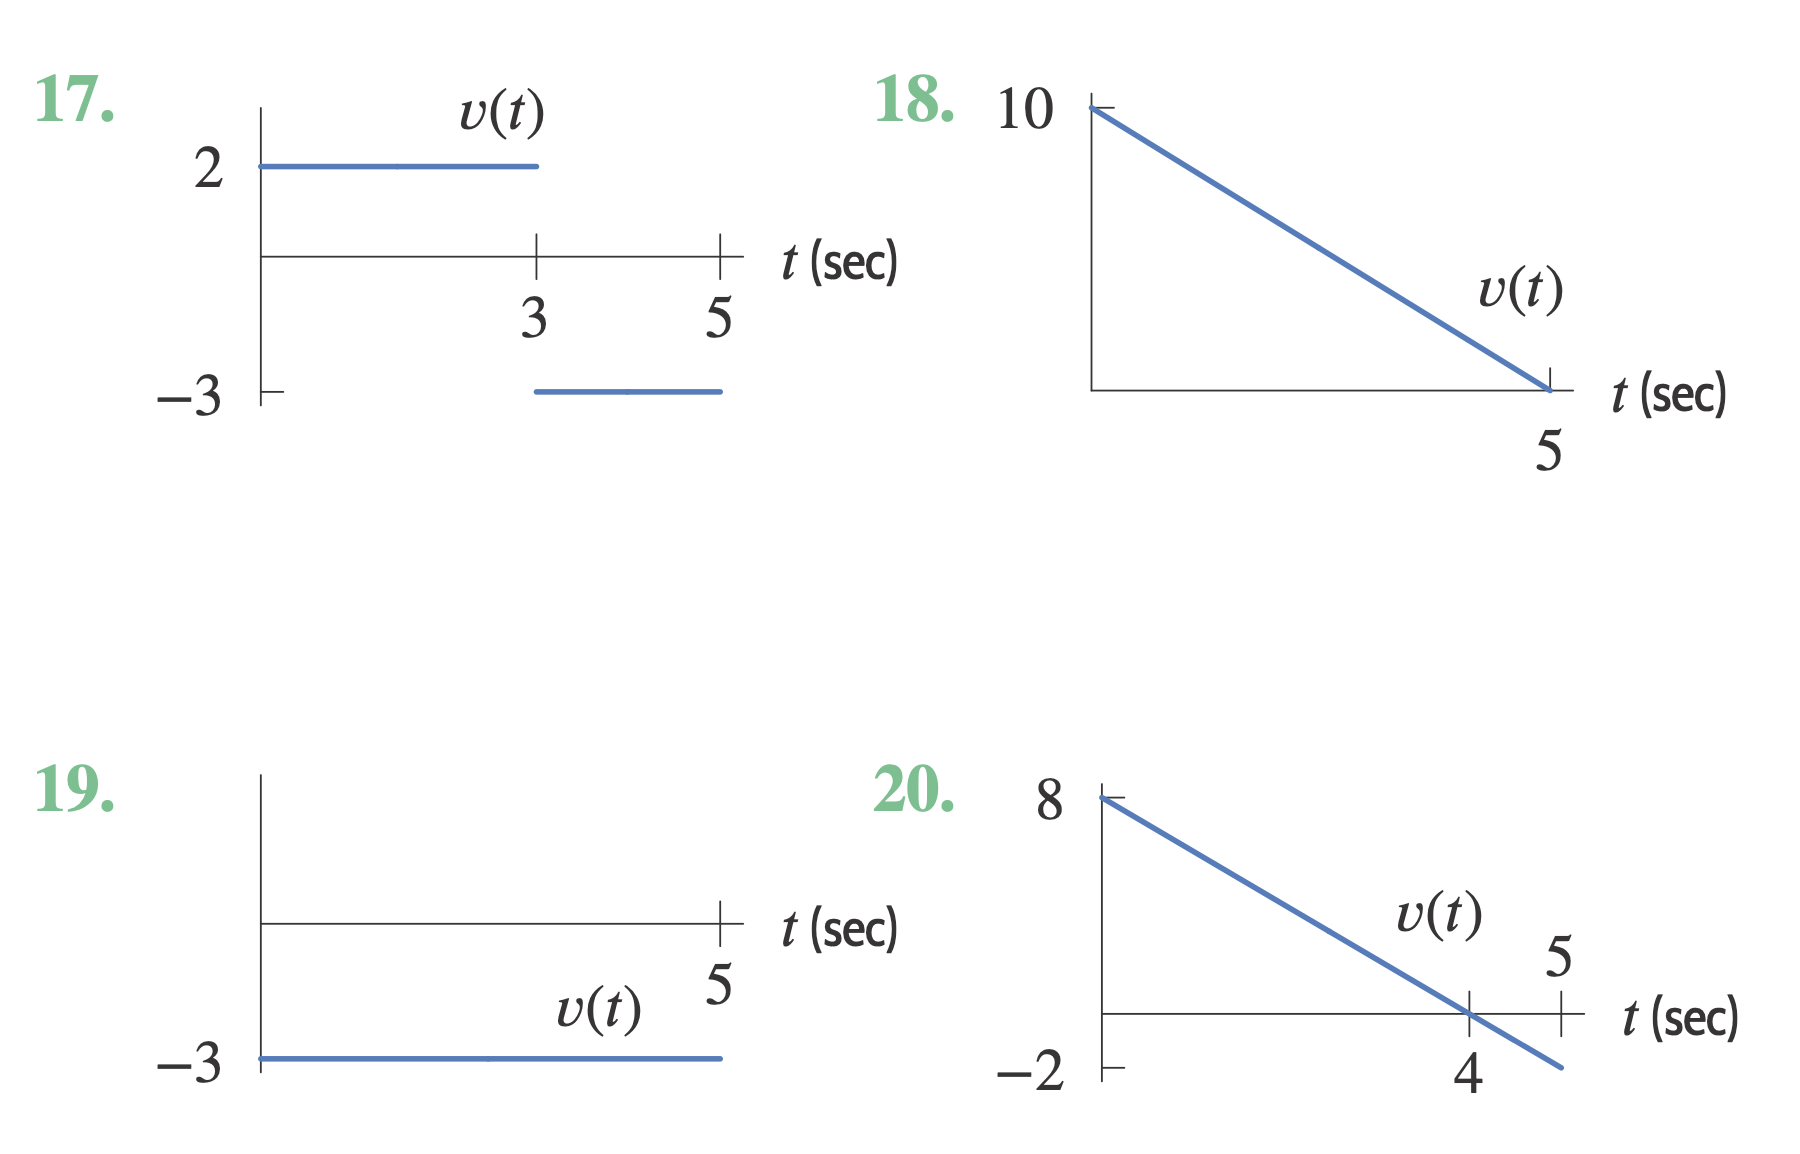
\includegraphics[scale=0.4]{Figures/graphs.png}
  \end{center}
  \begin{solution}
    \begin{enumerate}
    \item[17.] Change in position = \(3\cdot 2 + 2 \cdot(-3) =
      0\) cm. Total distance = \(3 \cdot 2 + 2 \cdot 3 = 12\) cm.
    \item[18.] Change in position = \(0.5 \cdot 10 \cdot 5 = 25\)
      cm. This is also the total distance traveled.
    \item[19.] Change in position = \(5 \cdot (-3) = -15\) cm. Total
      distance = \(15\) cm.
    \item[20.] Change in position = \(0.5 \cdot 8 \cdot 4 + 0.5 \cdot
      (-2) \cdot 1 = 16-1 = 15\) cm. Total distance = \(17\) cm.
    \end{enumerate}
  \end{solution}
\question The velocity of an object for \(0 \leq t \leq 8\) is shown
  below. Calculate the following estimates of the distance the object
  travels between \(t=0\) and \(t=8\) and indicate whether each is an
  upper or lower estimate of the distance traveled. 
  \begin{parts}
  \part A left sum with \(n=2\) subdivisions
  \part A right sum with \(n=2\) subdivisions
  \end{parts}
  \begin{center}
    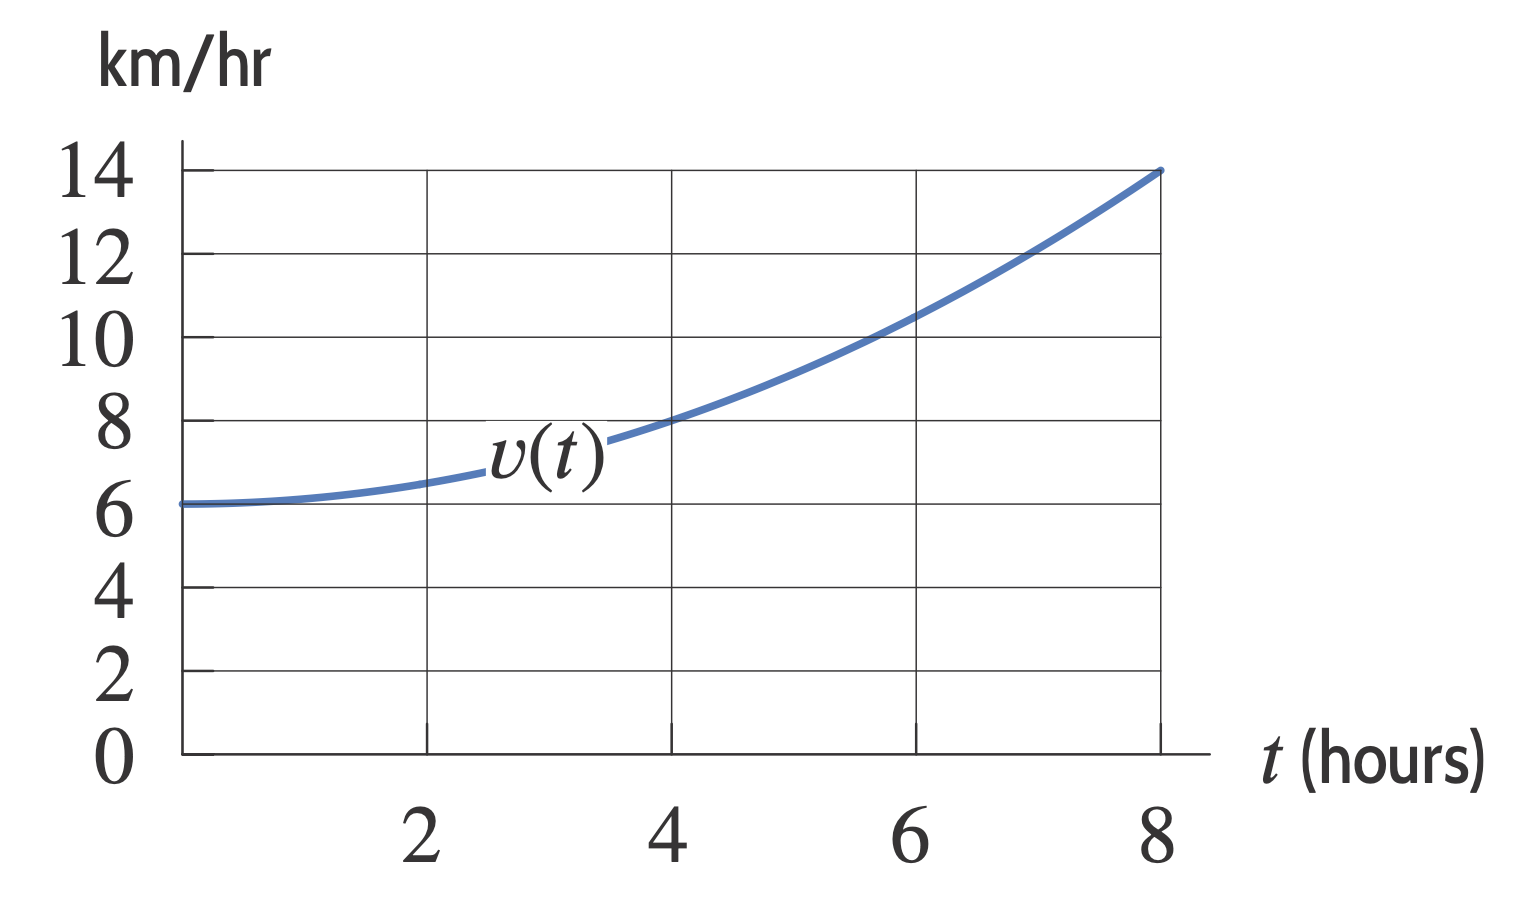
\includegraphics[scale=0.3]{Figures/figure514.png}
  \end{center}
  \begin{solution}
    \begin{enumerate}[(a)]
    \item \(2(6+8) = 28\) is a lower estimate
    \item \(2(8+14) = 44\) is an upper estimate
    \end{enumerate}
  \end{solution}
\question Find the difference between upper and lower estimates of the distance traveled at velocity $f(t)$ on the interval $a\leq t \leq b$ for $n$ subdivisions: $f(t) = e^{ - t^2 / 2 }$, $a=0$, $b=2$, $n=20$. 
  \begin{solution}
    Since \(f(0) > f(2)\), the difference in estimates will be
    \(n(f(a)-f(b)) = 20(e^0-e^{-4/2}) = 20(1-e^{-2})\). 
  \end{solution}
\question At time \(t\), in second, your velocity, \(v\), in
  meters/second, is given by \[
    v(t) = 1+t^2 \text{ for }0 \leq t \leq 6
  \]
  Use \(\Delta t = 2\) to estimate the distance traveled during this
  time. Find the upper and lower estimates, and then average the two.
  \begin{solution}
    We compute \[
      v(0) = 1, v(2) = 5, v(4) = 17, v(6) = 37
    \]
    Then, a lower estimate is \(2(1+5+17) = 46\) meters and an upper
    estimate is \(2(5+17+37) = 118\) meters. The average is
    \(0.5(46+118) = 82\) meters.
  \end{solution}
\end{questions}
\end{document}
%%% Local Variables:
%%% mode: latex
%%% TeX-master: t
%%% End:
